\documentclass[]{article}
\usepackage{graphicx}
%opening
\title{Puck manual}
\author{}

\begin{document}

\maketitle

\begin{abstract}

\end{abstract}

\section{User Interface}

Puck's interface is composed of four panels(cf figure \ref{fig:screenshot}). 

\begin{enumerate}
\item the button panel
\item the package explorer
\item the node information panel
\item the console
\end{enumerate}

A normal work space for puck is composed by a folder containing java sources (1.4 or 1.5).
A file named \verb|decouple.pl| placed at the root of the work space.

Optionally the following input can also be given to puck by placing them at the root of the work space :
\begin{itemize}
\item \verb|jar.list| : A file containing a list of absolute paths to jar archives (one per line), if the sources requires external libraries to compile.
\item \verb|api_nodes| : A list of elements of the java standard library that you wish to see displayed on the graph.
\end{itemize} 

The most simple use case, if you have a work space containing the above mention files with the default name and path, you just have to select it with the
 \verb|Work space| button\footnote{puck takes the directory from where it was open as its default work space} and press \verb|Dot it !|.



\begin{figure}
\centerline{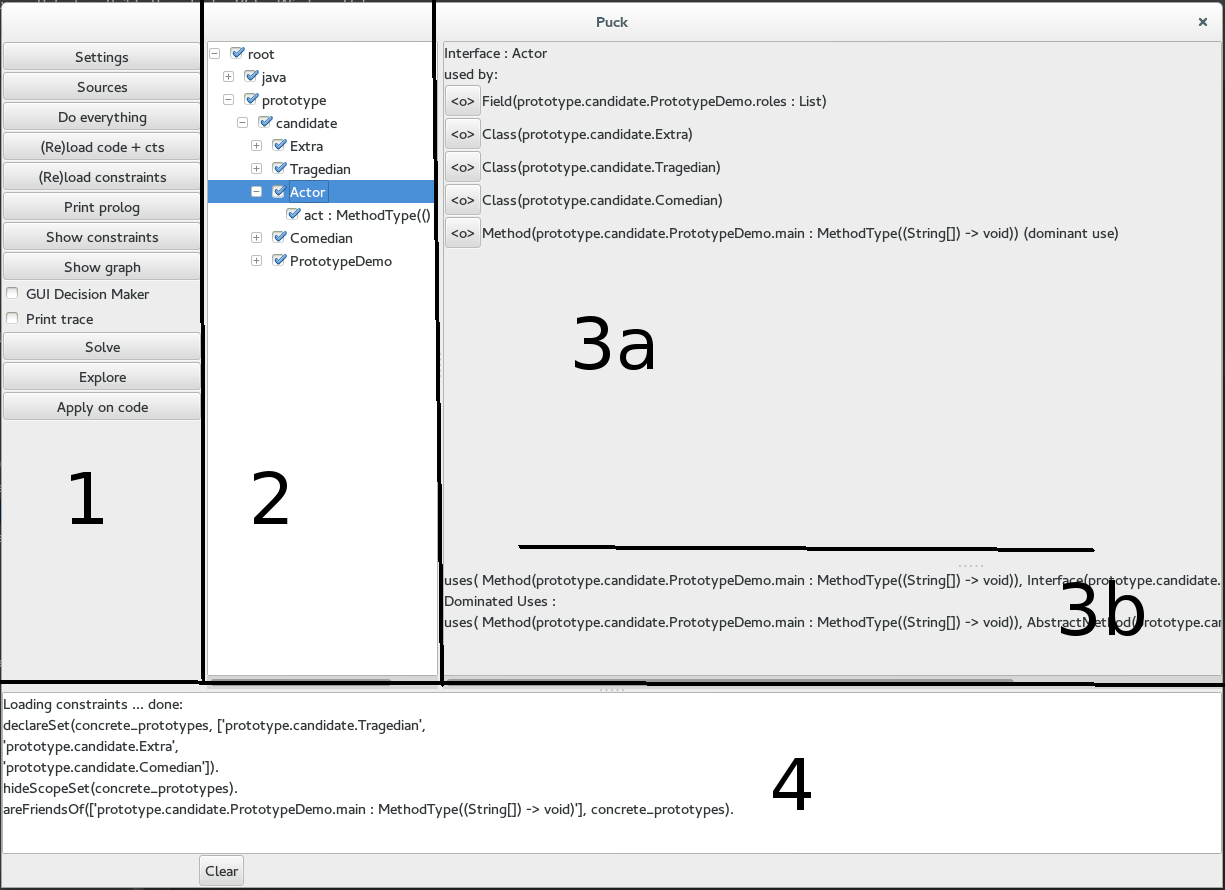
\includegraphics[keepaspectratio, width=1.7\textwidth]{screenshot.png}}
\caption{Screenshot of main panel of puck}
\label{fig:screenshot}
\end{figure}
 
\section{Puck's Architecture}
Puck's architecture is composed of the following packages : 
\begin{itemize}
\item \verb|puck|\\
	root package, contains only the Front object
\item \verb|puck.graph|
\item \verb|puck.graph.backTrack|
\item \verb|puck.graph.constraints|
\item \verb|puck.gui|
\item \verb|puck.gui.decisionsFrames|
\item \verb|puck.javaAG|
\item \verb|puck.javaAG.nodeKind|
\item \verb|puck.search|
\item \verb|puck.util|\\
This package contains 
\begin{itemize}
\item a generic breadth first iterator for trees
\item a mini logger framework
\item some basic file helper functions and a timer
\end{itemize}

\end{itemize}


\end{document}
